\documentclass{VRARWorkshop}

\usepackage[utf8]{inputenc}
\usepackage[T1]{fontenc}
\usepackage[hidelinks]{hyperref}

\title{Creating an augmented reality system to support manual non-destructive ultrasonic testing of metal pipes and plates}

\authors{Robert Deppe, Oliver Nemitz, Jens Herder}

\affiliations{~}
% TODO: Correct affiliations

\abstract{
The aim of this paper is to describe the application of augmented reality technology in non–destructive testing of products of the metal–industry and a prototype created in the course of a bachelor--thesis.
The prototype is created with hard– and software, that is usually employed in the gaming industry, and delivers positions for creating c–-scans.
Using the ZEDmini in combination with the HTC VIVE enables realtime visualisation of the probes path in the HMD, as well as the setting of virtual markers on the specimen.
As a part of the implementation the downhill–simplex optimization–algorithm is implemented to fit the specimen to a cloud of recorded surfacepoints.
The accuracy is statistically tested and evaluated with the result, that the VIVE–trackingsystem is accurate up to ca. 1–2 millimeters in well lit conditions.
This paper is of interest not only for research–institutes of the metal–industry, but also for any areas of work, in which the enhancement with augmented–reality is possible.
}

% Give some keywords
\keywords{
Nondestructive Testing,
Ultrasonic,
Augmented Reality,
Tracking,
Stereocamera,
HTC VIVE,
ZED--mini,
NDT,
ZfP,
AR
}

\begin{document}

\section{Introduction}

\begin{figure}[h!]
    \begin{center}
        \includegraphics[width=79mm]{images/US-workspace.jpg}
        \caption{\label{fig:europipe} Workspace for manual ultrasonic-testing of steel pipeline pipes at Europipe in Mülheim an der Ruhr.}
    \end{center}
\end{figure}

\begin{figure}[h!]
    \begin{center}
        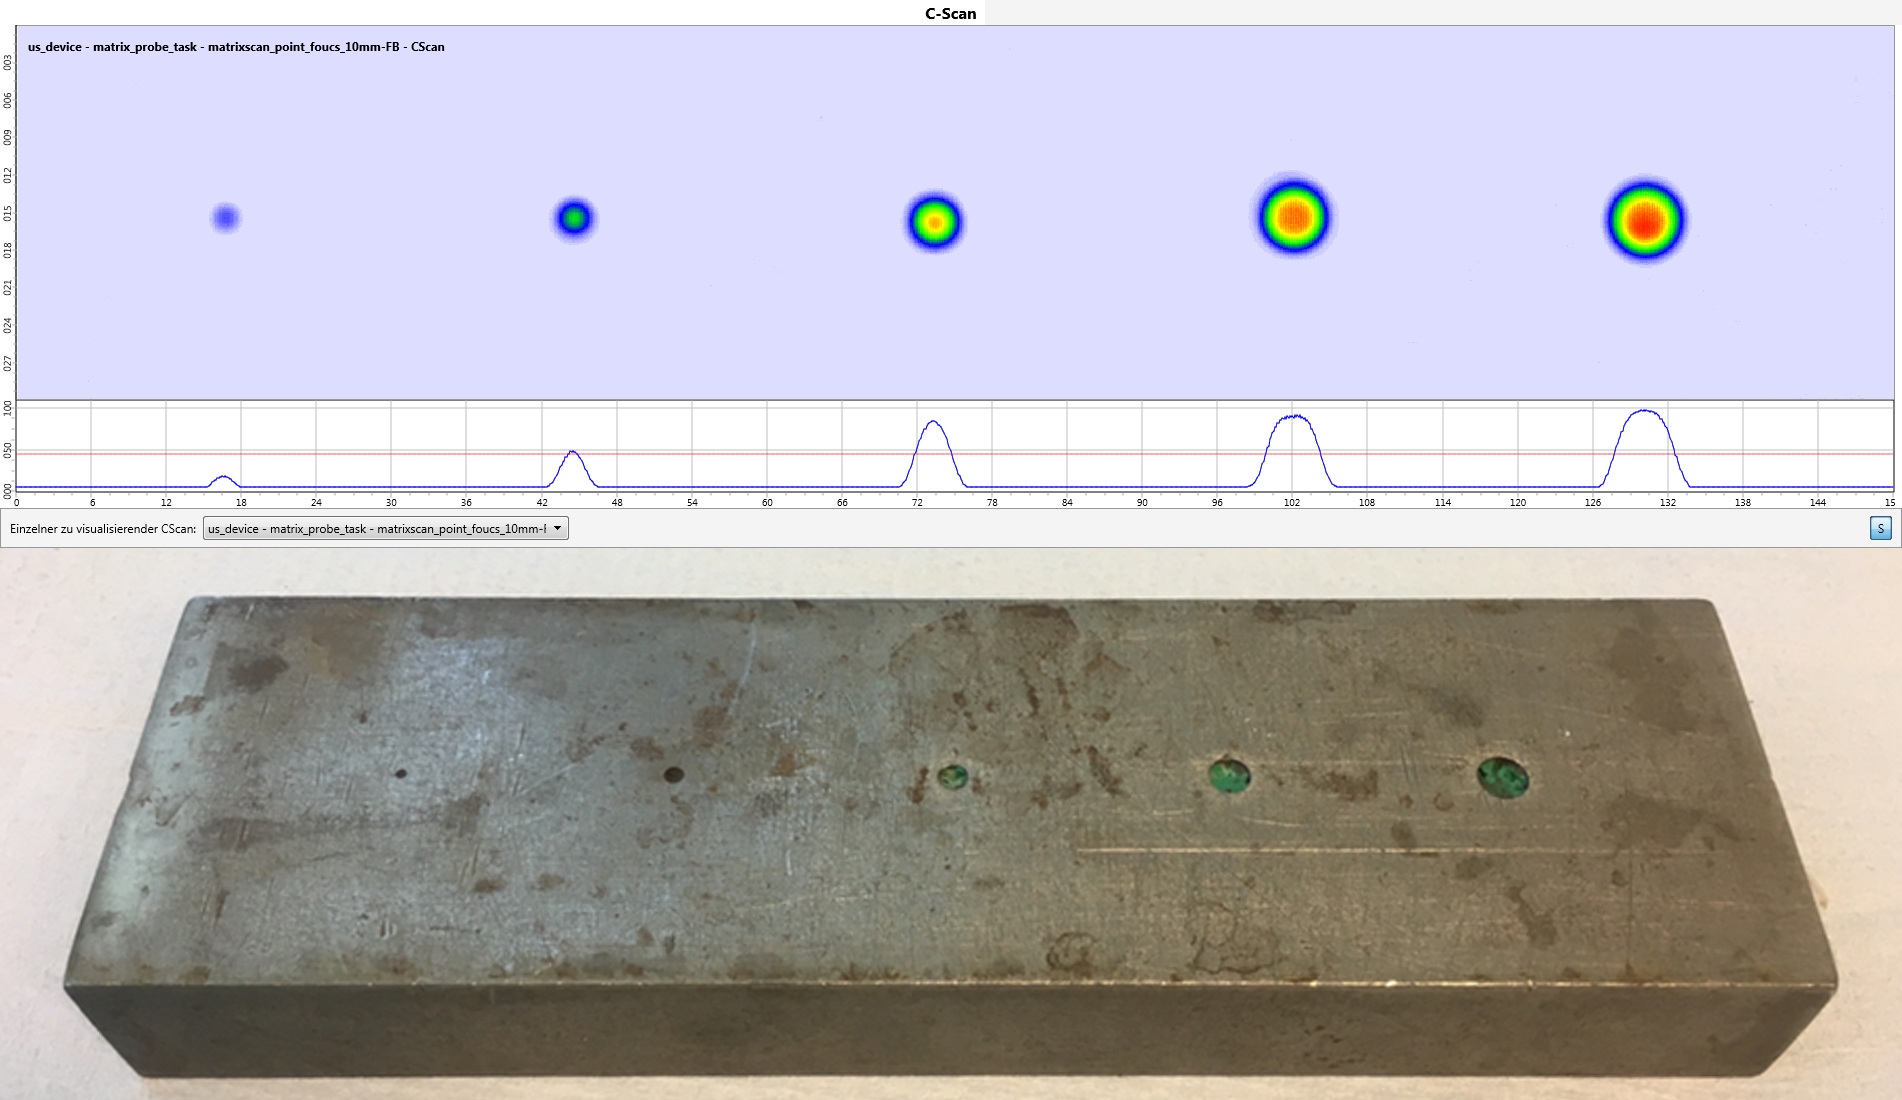
\includegraphics[width=79mm]{images/CScan.jpg}
        \caption{\label{fig:cScan} C--Scan with a resolution of 0,1\,mm}
    \end{center}
\end{figure}

\section{Related Research}
\cite{ARPat15}
\cite{ARClean}
\cite{schwerdtfeger_using_2008}
\cite{fadzil_design_2015}
\cite{walter_non-contact_2007}

\section{Basics of non-destructive ultrasonic testing of metal products}
\cite{deutsch_zfp_2010}
\cite{moles_introduction_2004}
\cite{olympus_Grundlagen}

\textcolor{red}{Soll noch ein Abschnitt zu den AR Grundlagen gemacht werden?}

\section{Description of the AR--application}

\section{Implementation}
\cite{dorner_virtual_2013}

\begin{figure}[h!]
    \begin{center}
        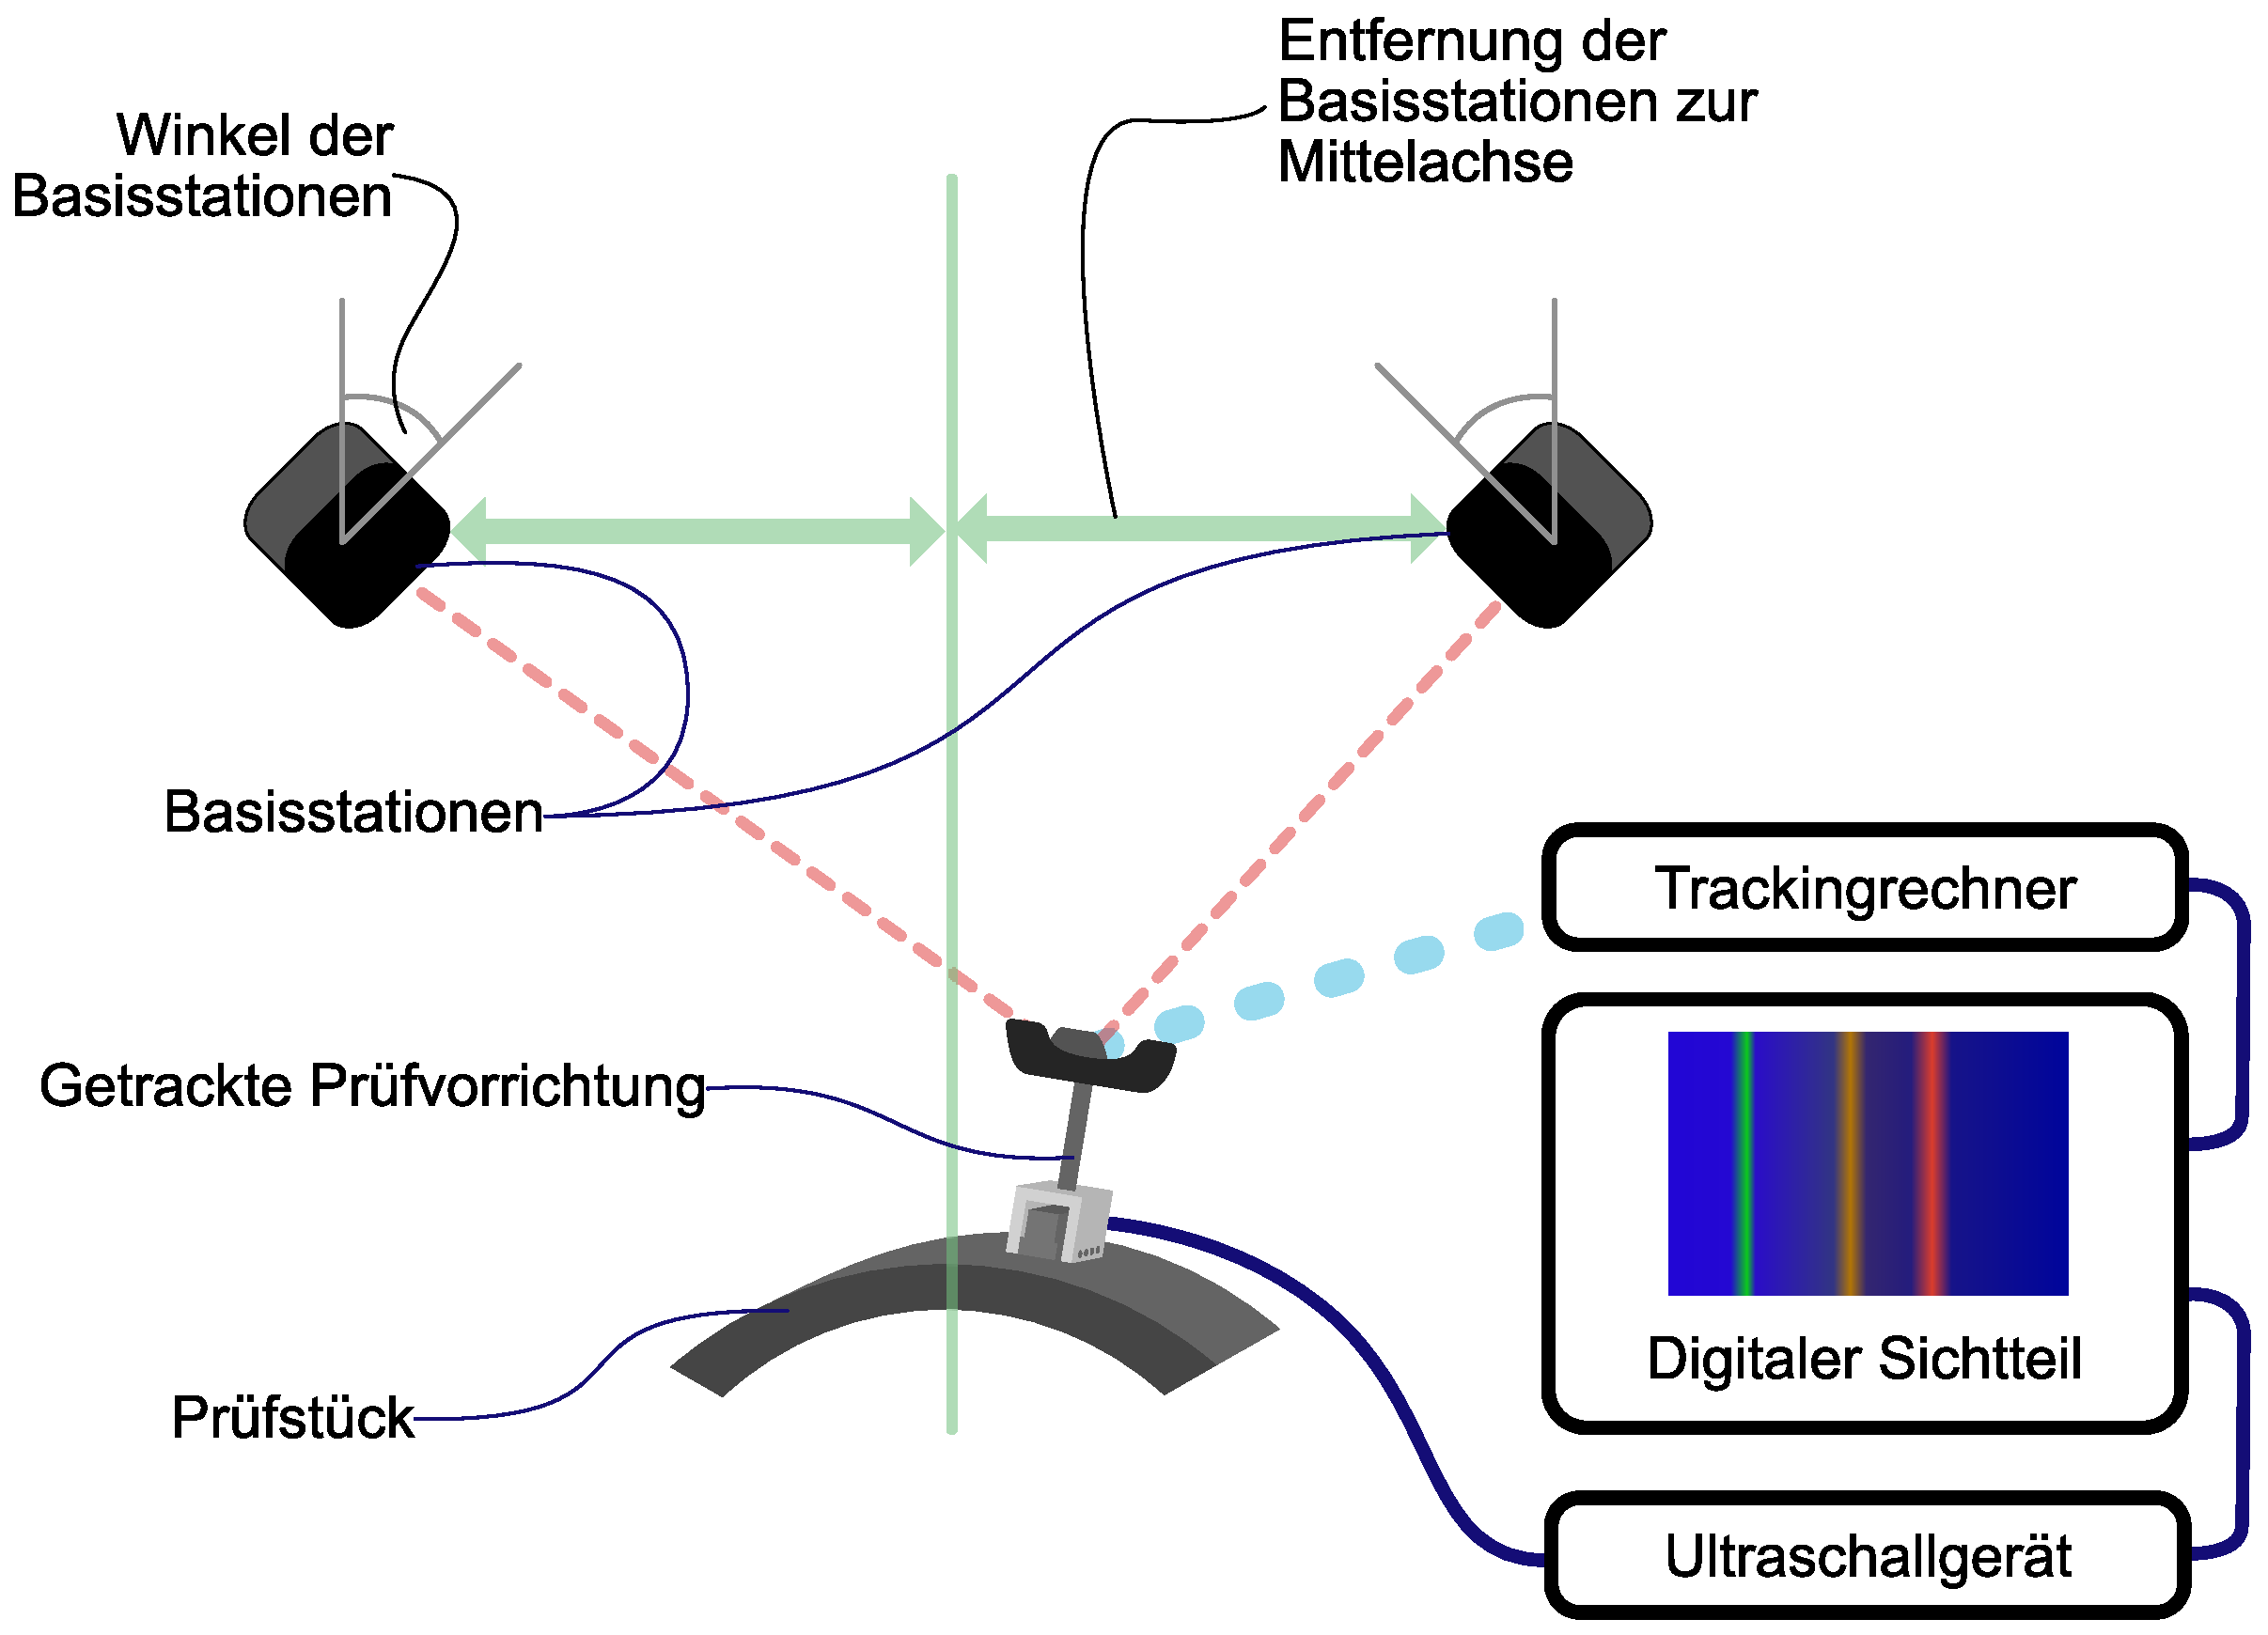
\includegraphics[width=79mm]{images/Setup.eps}
        \caption{\label{fig:Setup} Setup of the described AR-application. \textcolor{red}{Grafik muss noch übersetzt werden.}}
        % TODO: Grafik übersetzen
    \end{center}
\end{figure}

\subsection{Tracking of the ultrasonic probe}
The ultrasonic probe is tracked with the help of a attachable tracked \textit{VIVE}--Tracker.
This Tracker is attached to a mount, in which the ultrasonic probe is fixed.
The offset and orientation between the tracker and probe is applied in software by setting the virtual probe as a child transform of the tracker.

\begin{figure}[h!]
    \begin{center}
        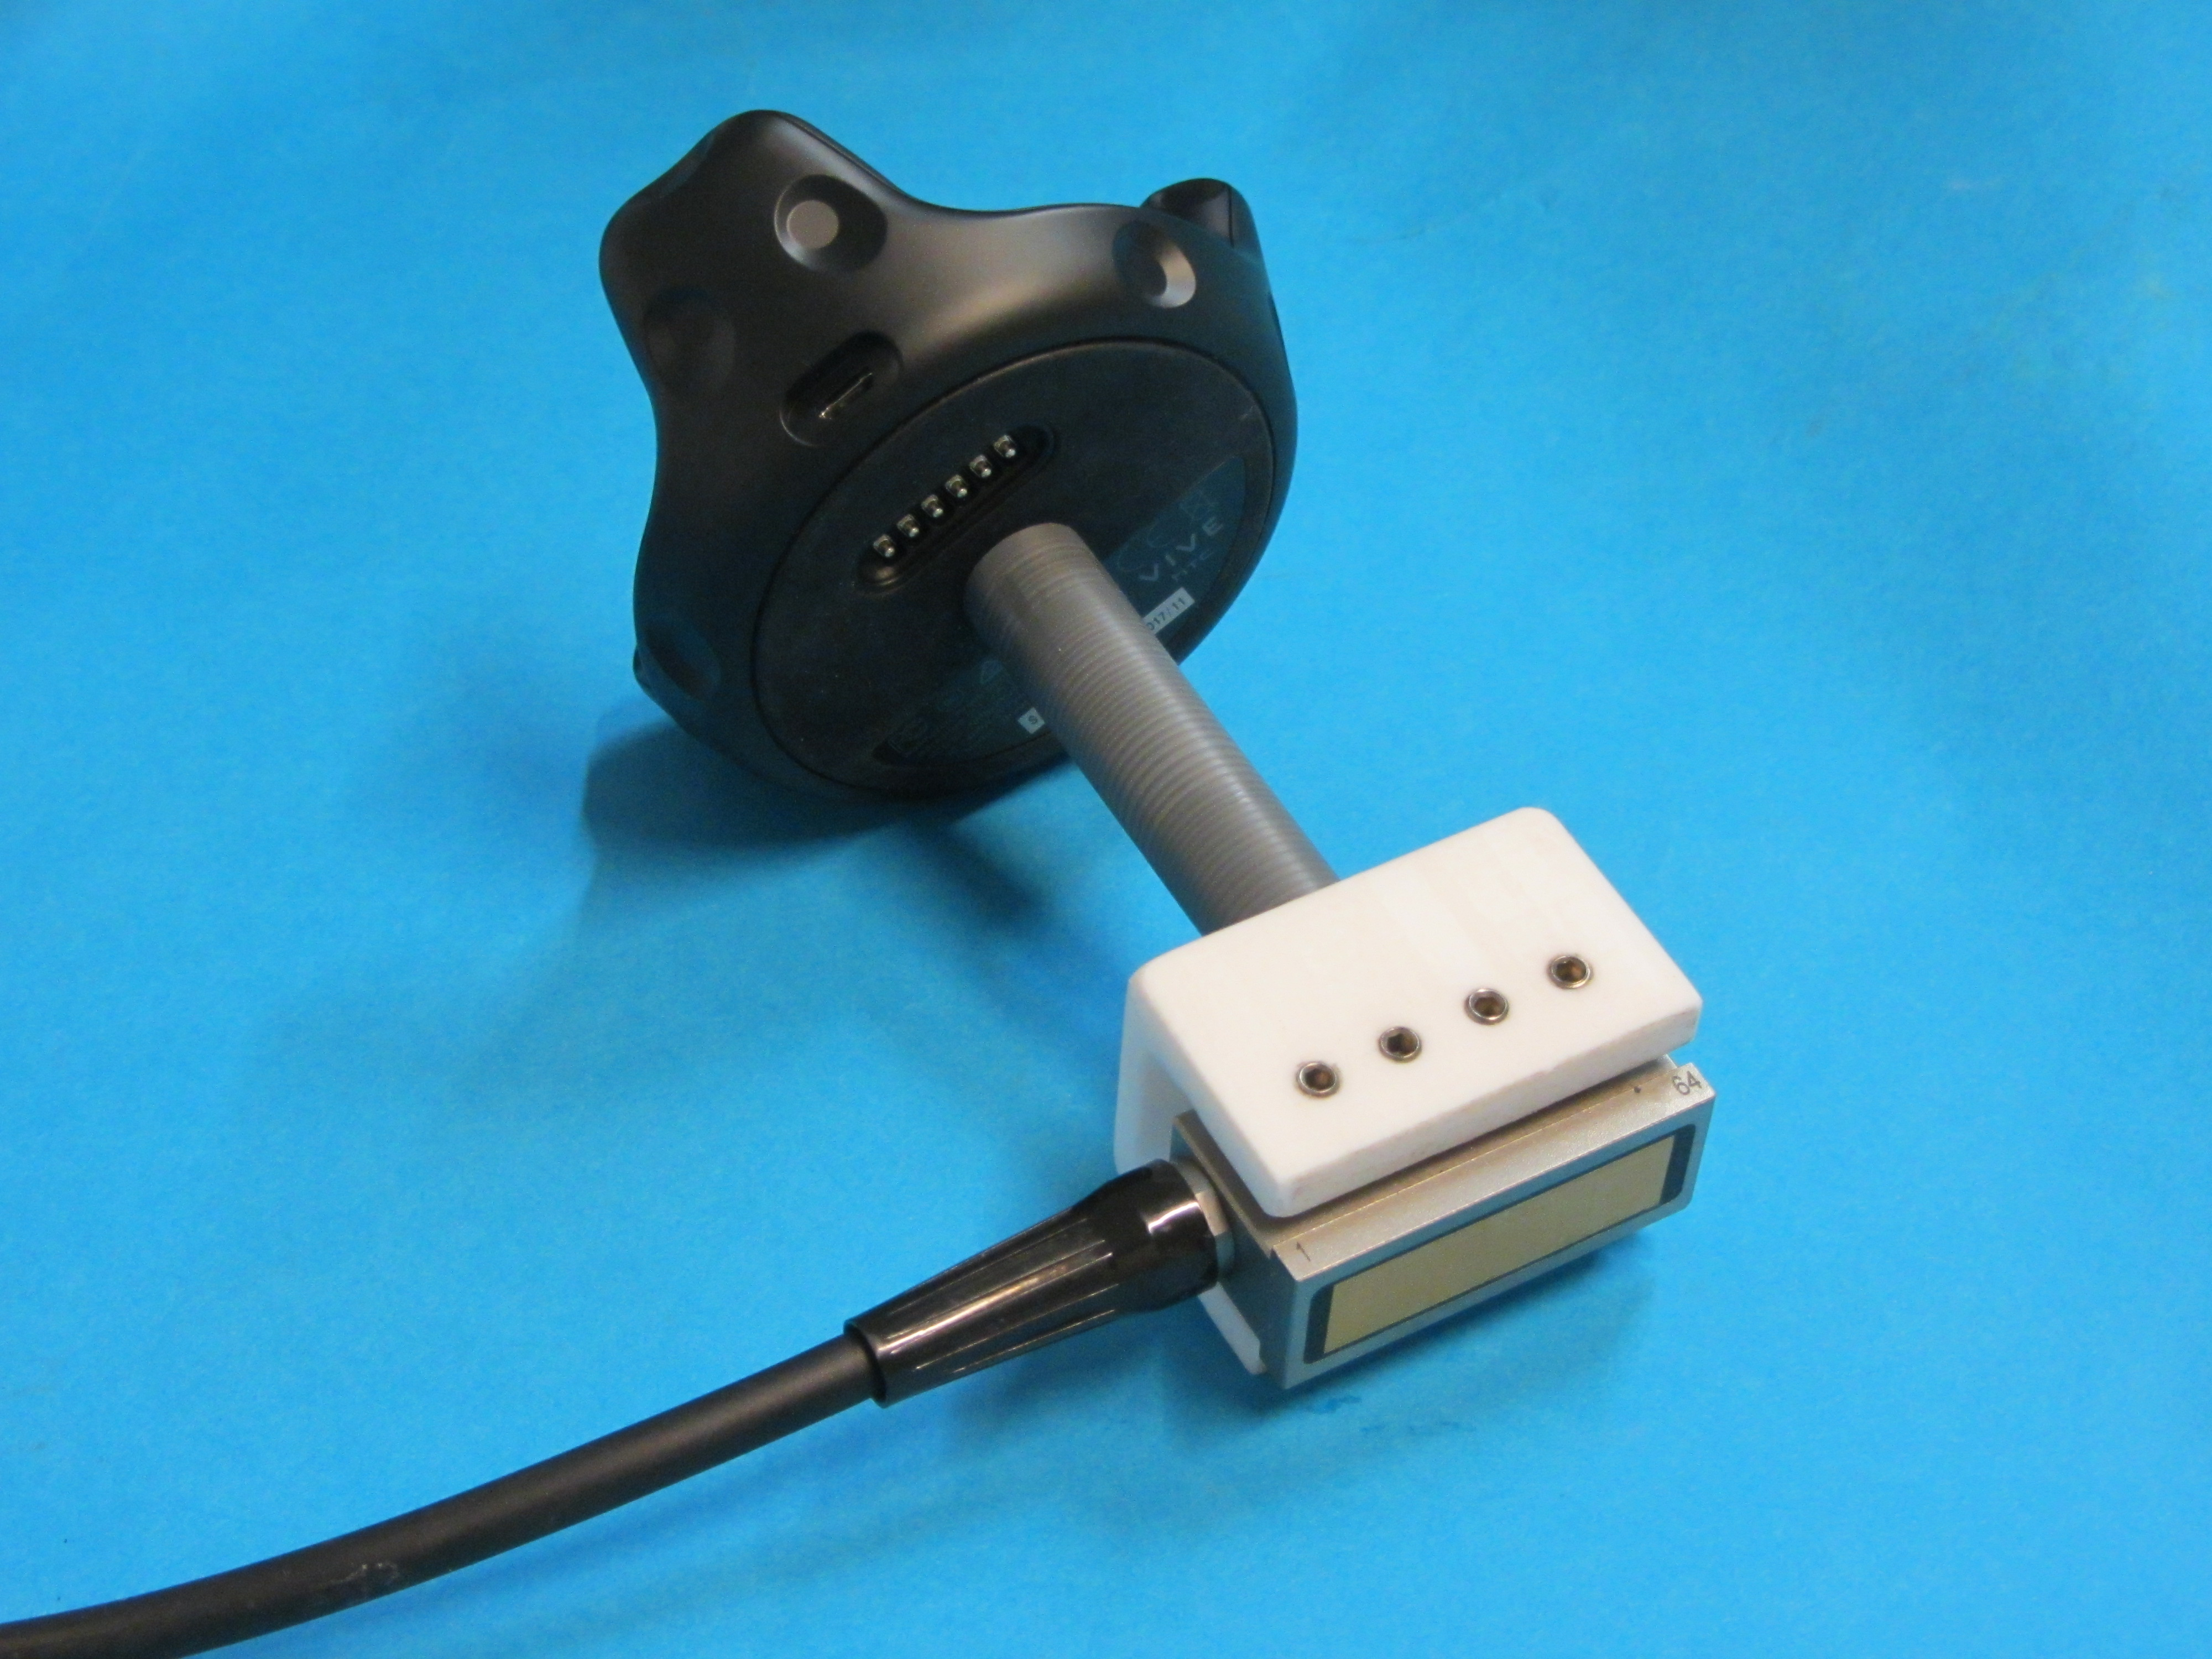
\includegraphics[width=79mm]{images/probemount.jpg}
        \caption{\label{fig:probemount} Probemount, that fixes \textit{VIVE--}Tracker to ultrasonic probe.}
    \end{center}
\end{figure}

\subsection{Detection of the coordinate system in worldspace}
The coordinate system of the surface to be measured is detected in two steps:
first a point--cloud of the surface is created by moving the tracked probe across it.
In the next step the parameters of the selected geometry in worldspace are calculated from this point--cloud using the Downhill--Simplex optimization by Nelder and Mead.
In a second step the used coordinate system is picked by placing the tracked probe at the desired origin and pressing the setup button.
As the specimen--geometry is already defined, only one more axis is required to define the orthogonal coordinate system.
this is done by placing the tracked probe on the X--Axis and pressing the setup button.

\subsection{Vizualisation of the trackingdata}

\begin{figure}[h!]
    \begin{center}
        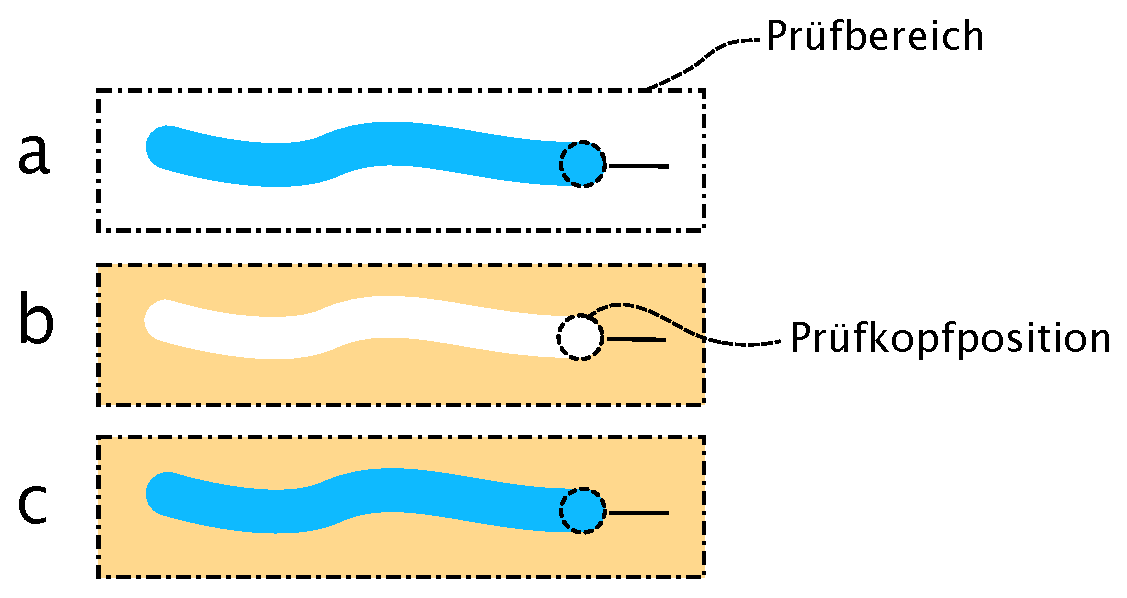
\includegraphics[width=79mm]{images/DrawVsErase.eps}
        \caption{\label{fig:DrawVsErase} Different methods to mark covered area.}
    \end{center}
\end{figure}

\subsection{Continuous and singular logging of position}

\section{Evaluation}

\begin{figure}[h!]
    \begin{center}
        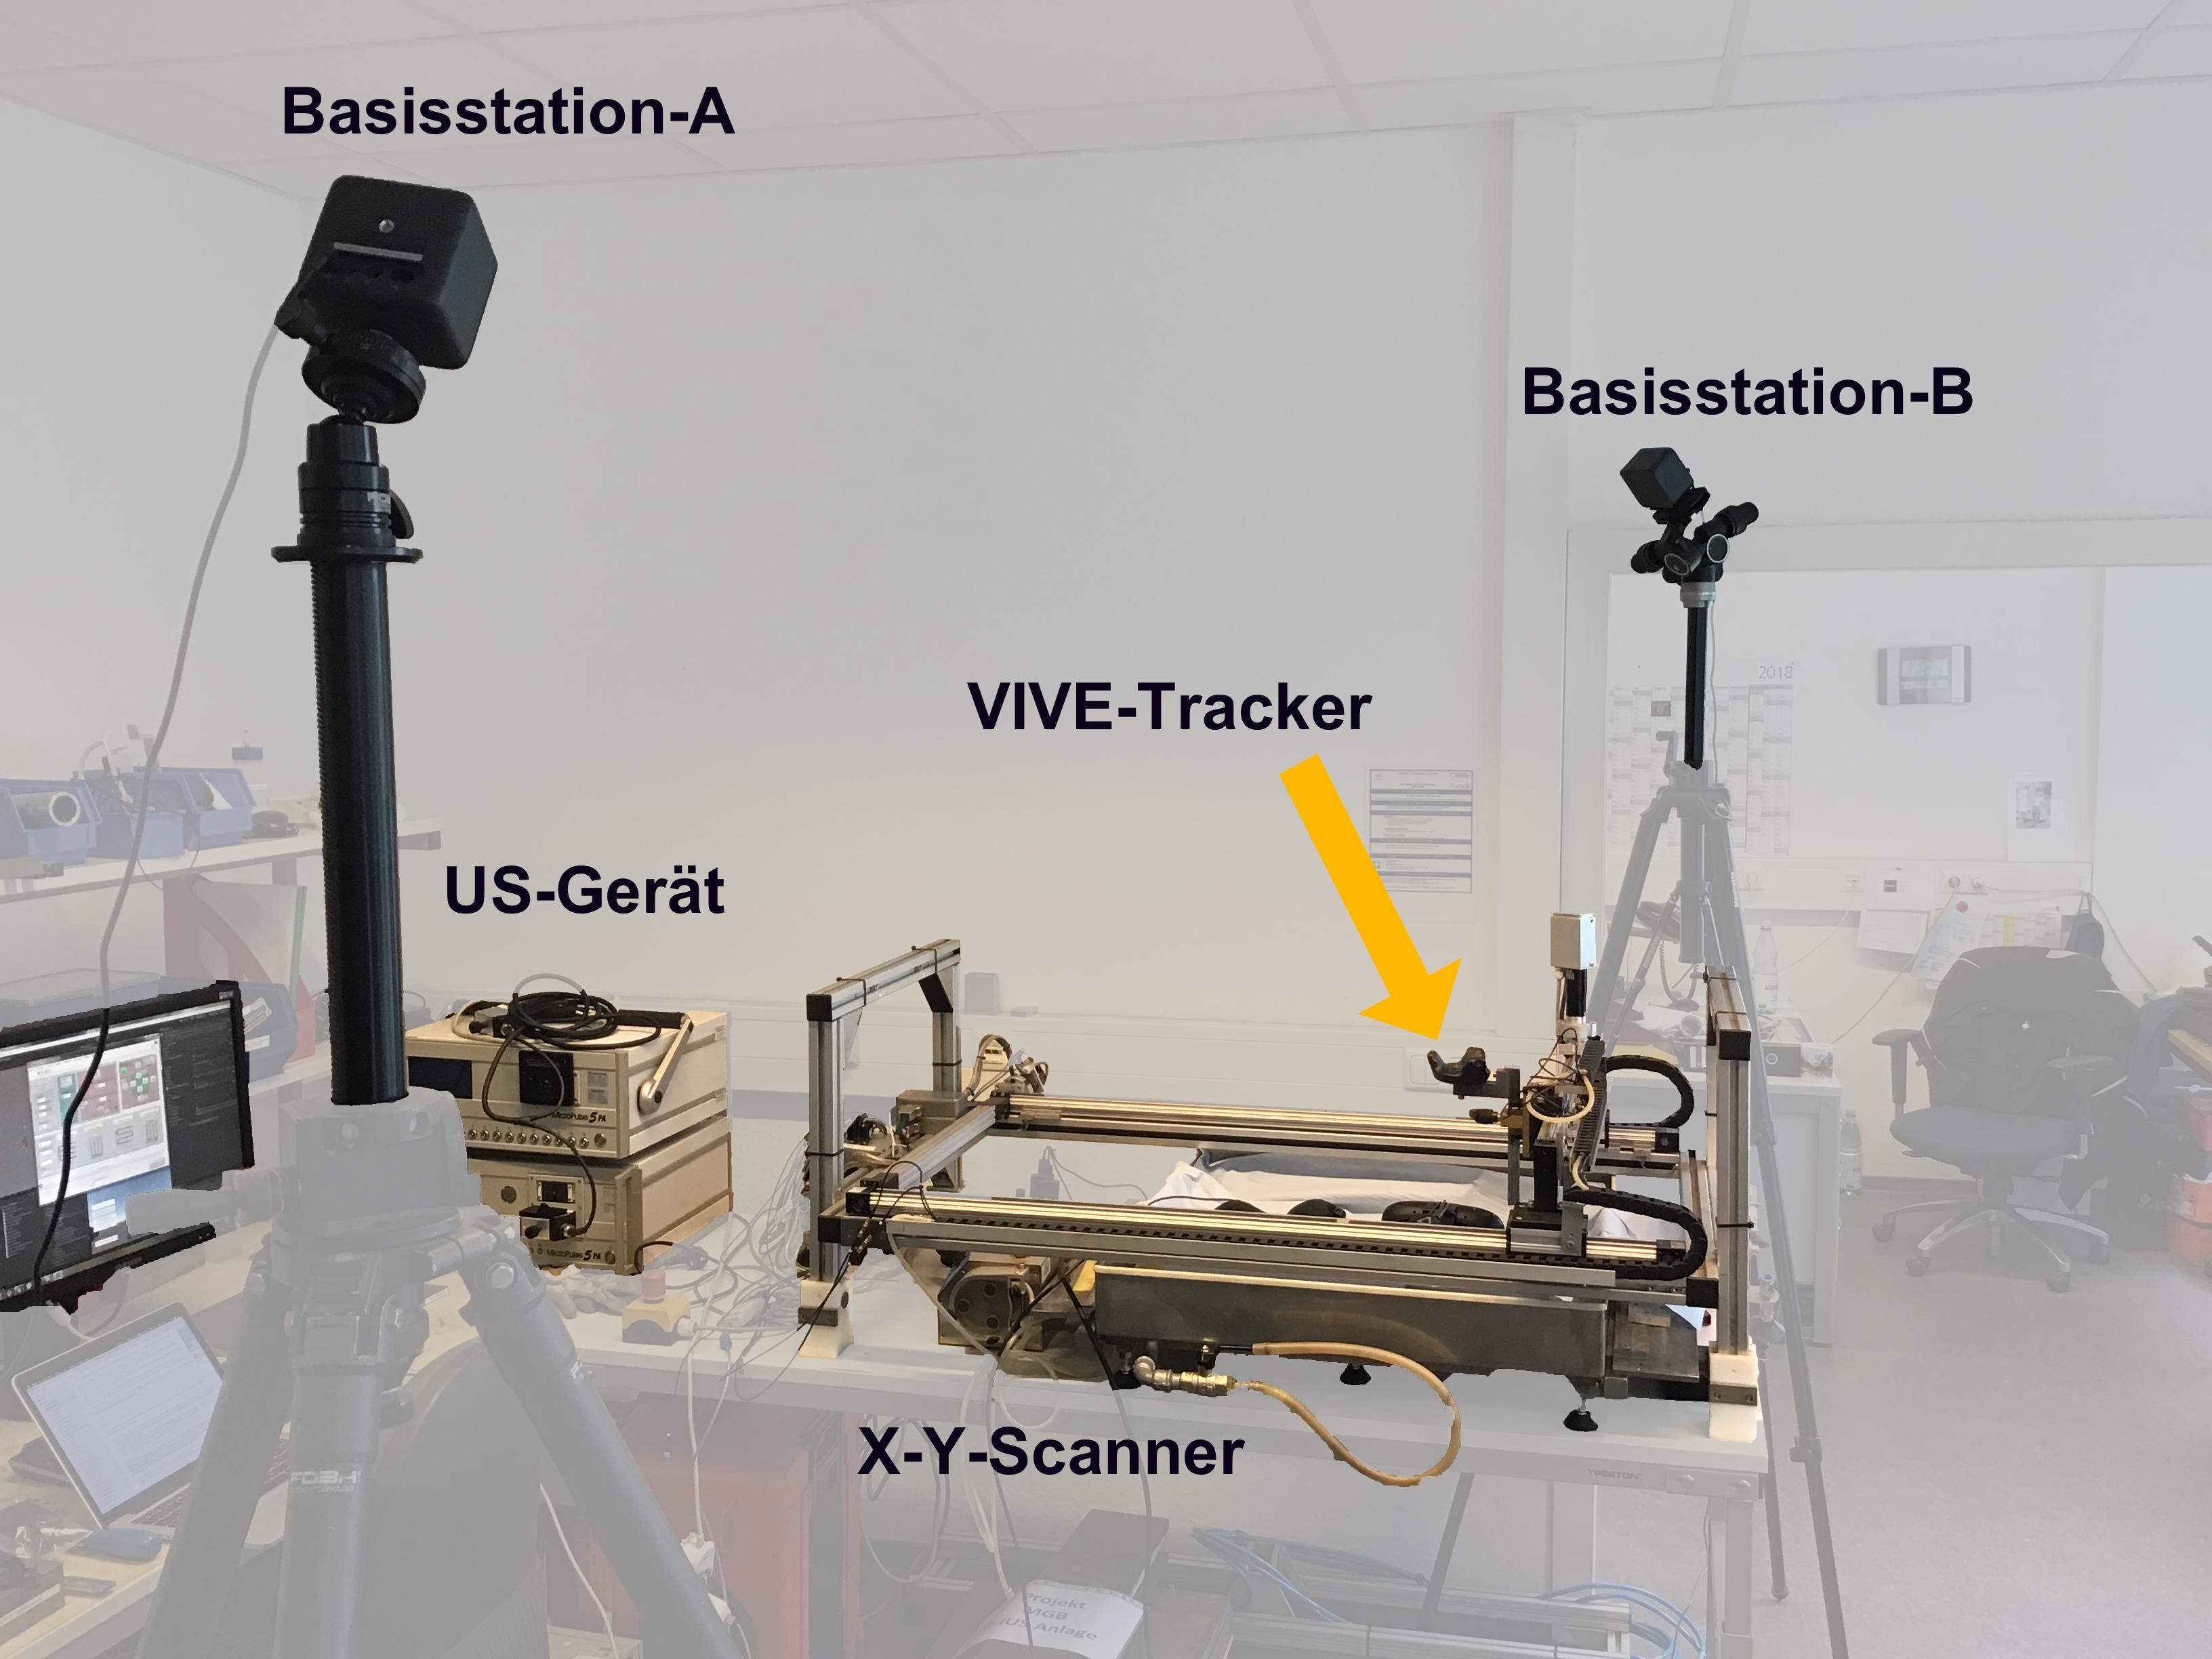
\includegraphics[width=79mm]{images/PrecisionMeasurement.jpg}
        \caption{\label{fig:precisionMeasurement} Setup for the evaluation of the \textit{VIVE}--Precision}
    \end{center}
\end{figure}

\begin{figure}[h!]
    \begin{center}
        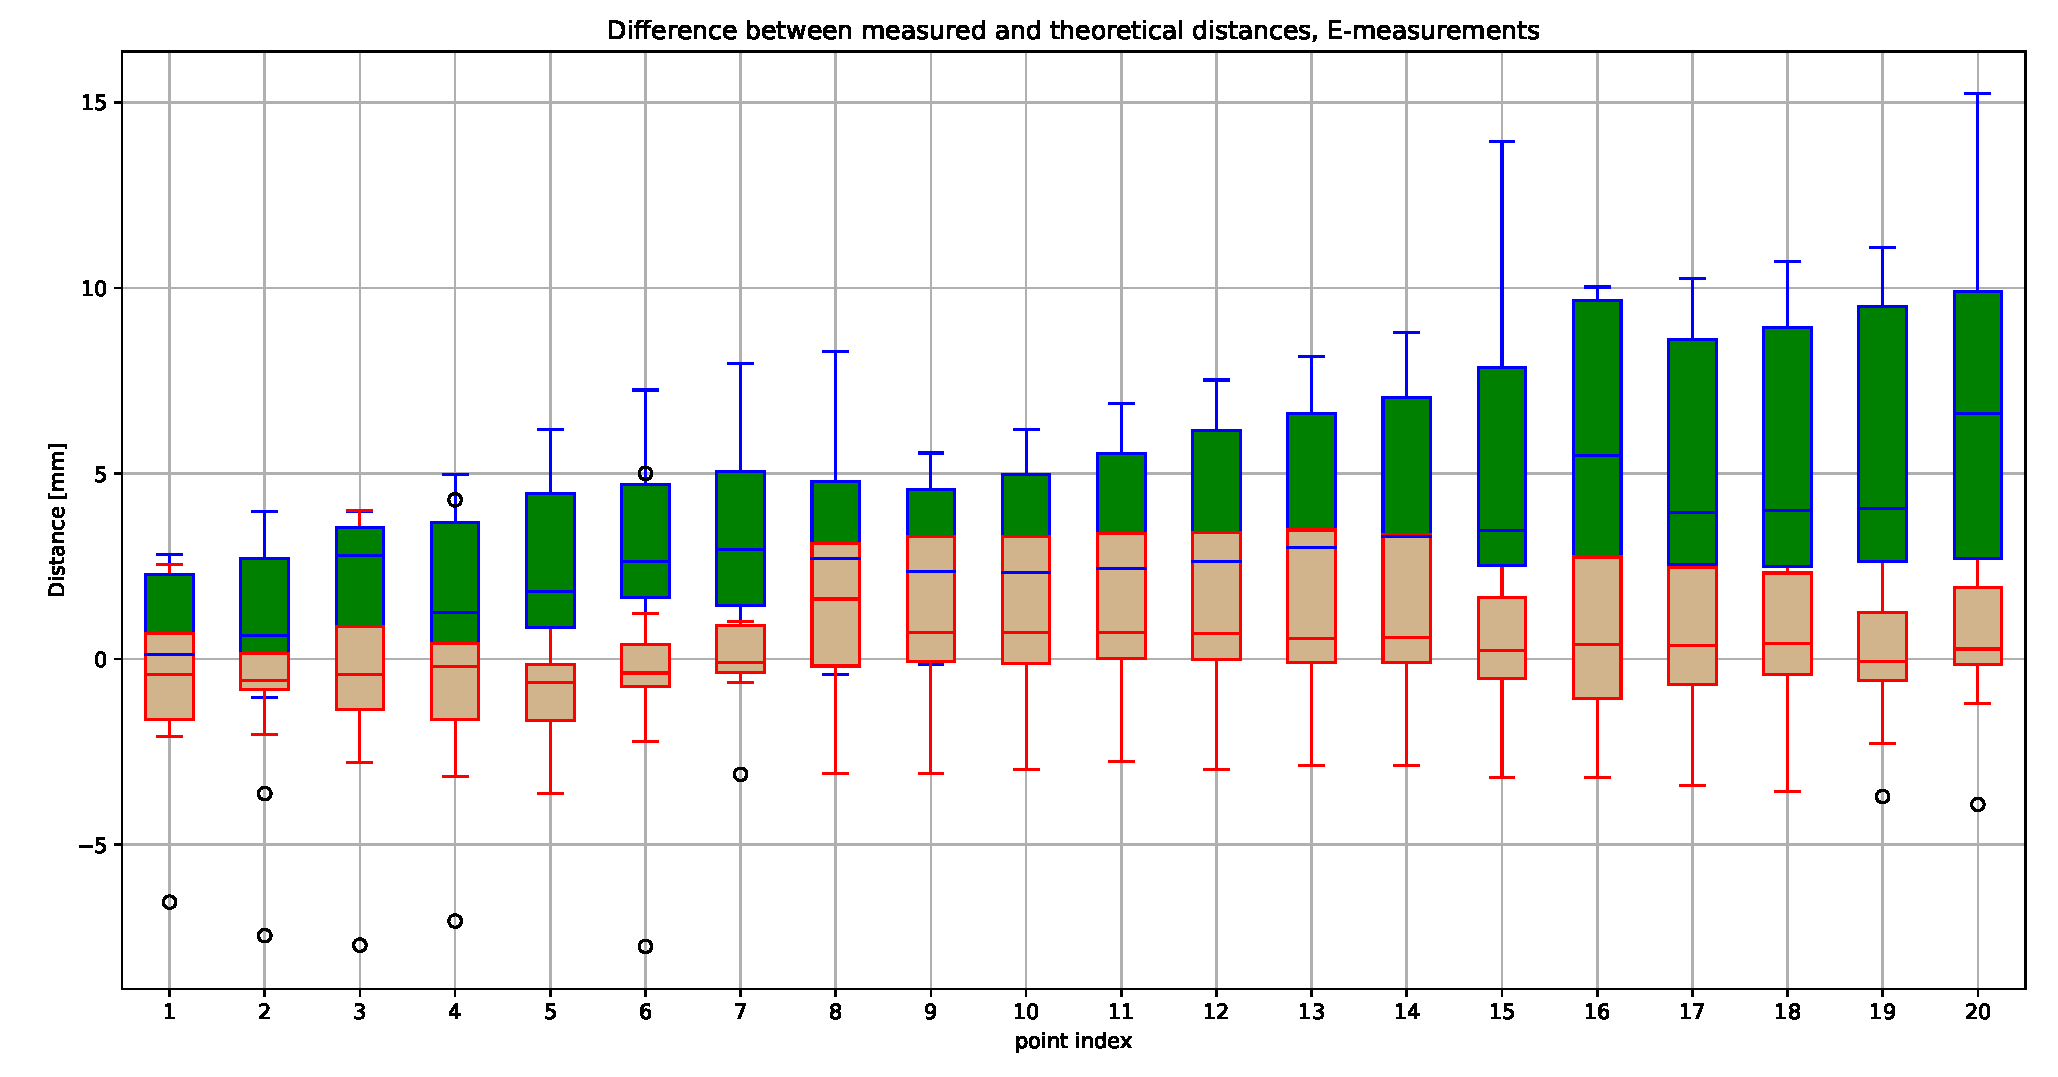
\includegraphics[width=79mm]{images/distancesBoxplot-E.eps}
        \caption{\label{fig:boxplotE} Difference between measured and theoretical distances to the reference point at the E--Positions.}
    \end{center}
\end{figure}

\begin{figure}[h!]
    \begin{center}
        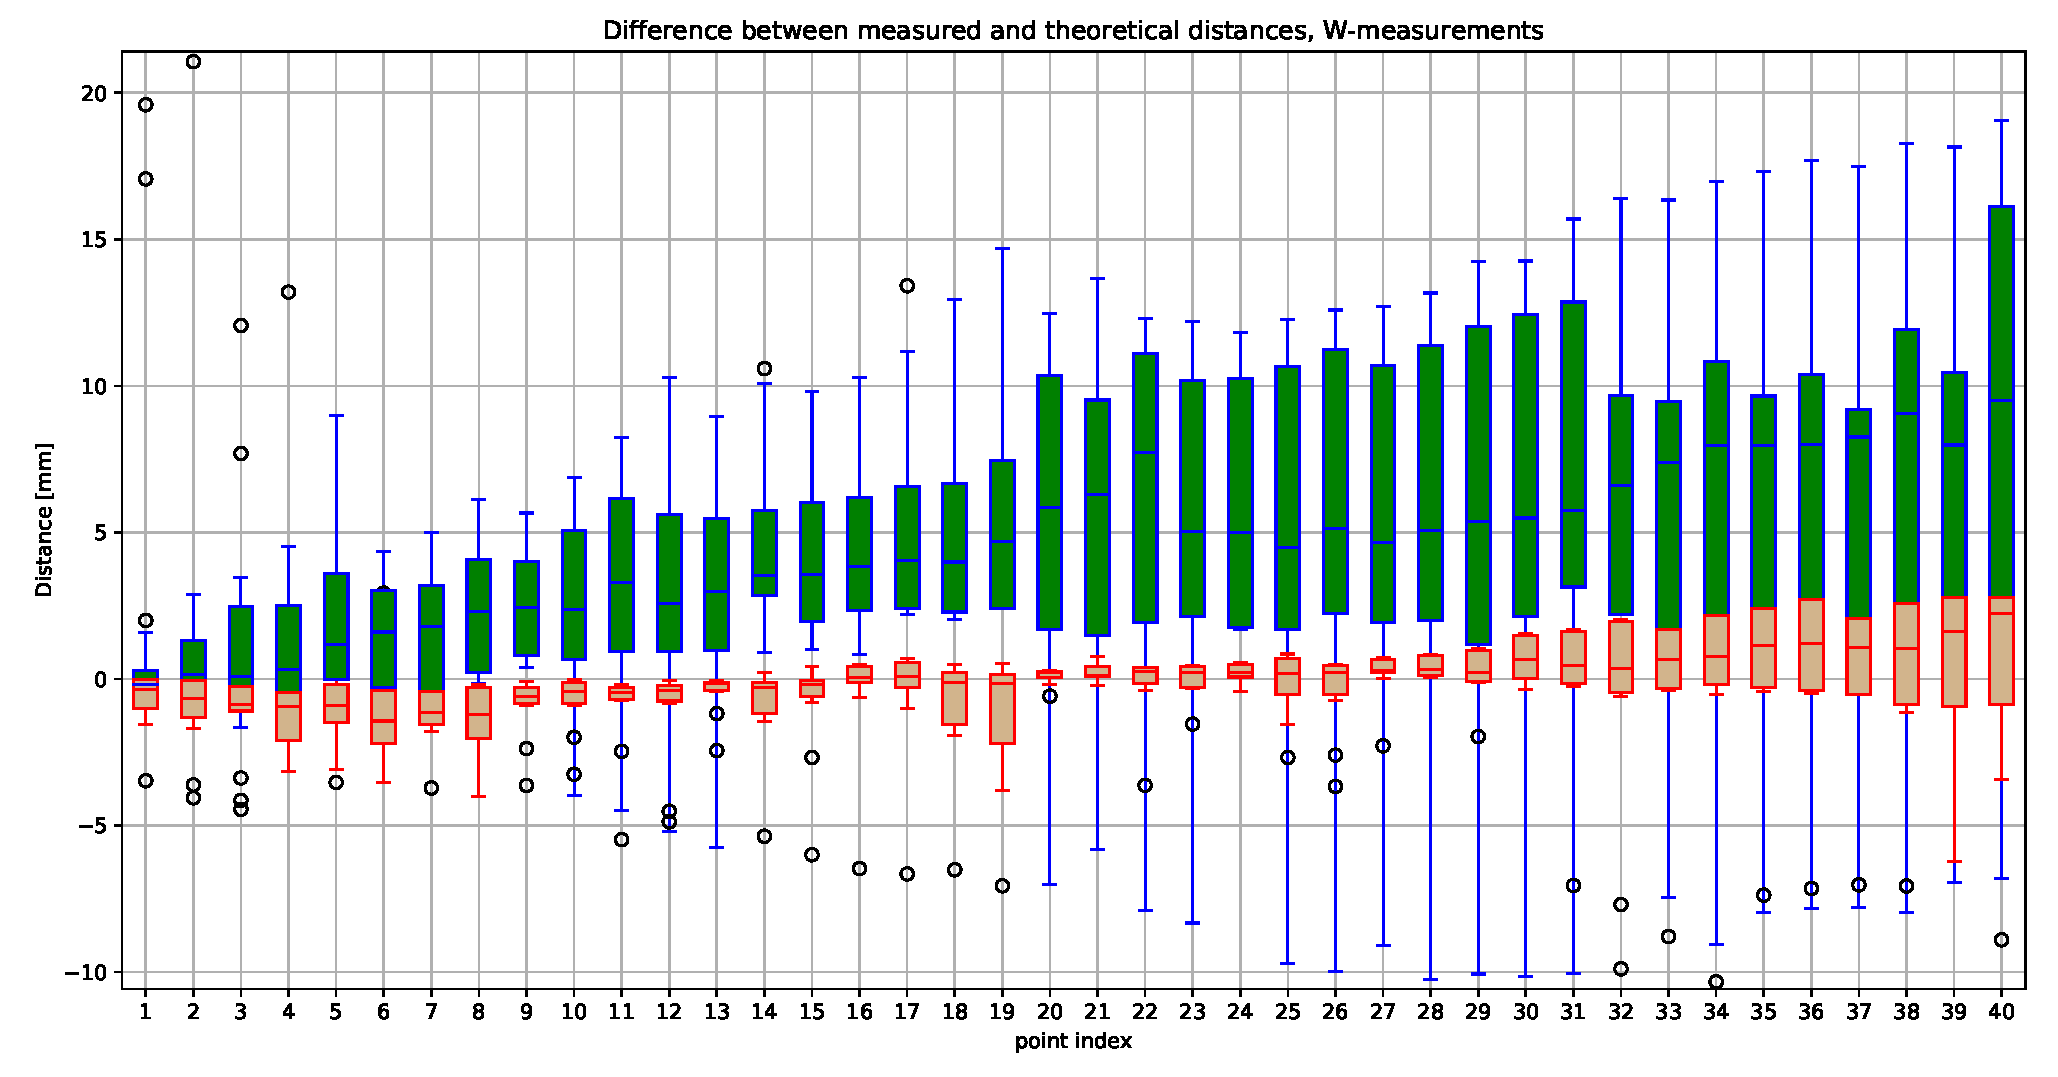
\includegraphics[width=79mm]{images/distancesBoxplot-W.eps}
        \caption{\label{fig:boxplotW} Difference between measured and theoretical distances to the reference point at the W--Positions.}
    \end{center}
\end{figure}

\section{Conclusion}

\VRARsetbibstyle
\bibliography{VRARTeXample}

\end{document}
